\documentclass[12pt]{article}

\usepackage{algorithmic}
\usepackage{amsmath}
\usepackage{graphicx}
\usepackage{hyperref}
\usepackage{booktabs}

\begin{document}

\title{CSI709 Midterm \\
Problem 1}
\author{
        Geoffrey Ulman \\
        George Mason University\\
}
\date{\today}

\maketitle

\section{K-Means Clustering}

The results of the k-means clustering performed on 84 samples of fiduciary point data (after centering the data and calculating \(dx\) and \(dy\) offsets from the average centered grid) is included in Table \ref{gini}.

\begin{figure}
\begin{equation}\label{eq_gini}
\begin{aligned}
\sum_{j=1}^{k} \hat{p}_j\left ( 1 - \hat{p}_j \right )
\end{aligned}
\end{equation}
\caption{Gini Index Definition}
\end{figure}

In addition to listing the names of the people associated with the data elements assigned to each cluster, Table \ref{gini} lists the Gini Index of the cluster. The Gini index is a measure of the purity of a grouping which is often employed when constructing classification trees. Let \(k\) be the number of classes (the total number of different people present in the cluster) and \(\hat{p}_j\) be the percentage of the cluster consisting of class \(j\), then the Gini Index is given by Equation \ref{eq_gini}. A Gini index of \(0.0\) indicates a completely pure cluster with only one class. Higher Gini index values indicate increasingly impure classes.

It is clear from Table \ref{gini} that there is structure in the data (a large number of classes have \(0.0\) to \(0.4\) Gini Index and have at most \(1\) data value not like the others). However, there are also large clusters with many different values. This indicates that perhaps results could be improved by rebreaking those large clusters. Note that because the k-means clustering routine starts with random initial clusters, the values in Table \ref{gini} only represent one possible clustering result.

\begin{table}\scriptsize
\begin{center}
\caption{Contents and Gini Index of K-Means Clusters}
\begin{tabular}{lr}
\\
\toprule
Cluster & Gini Index \\
\midrule
fjem0,fjem0,fjem0,fjem0 & 0.000 \\ \midrule
fadg0,fadg0 & 0.000 \\ \midrule
mstk0,mgwt0 & 0.500 \\ \midrule
fadg0,fedw0,fedw0 & \\
fedw0,fjem0,mpgl0 & 0.667 \\ \midrule
mtmr0,mtmr0,mtmr0 & \\
mtmr0,mtmr0,mdab0 & 0.278 \\ \midrule
mrjo0,mrjo0,mrjo0 & 0.000 \\ \midrule
mwbt0,mwbt0,mwbt0 & \\
mwbt0,msjs1 & 0.320 \\ \midrule
mrcz0,mrcz0,mrcz0,mrcz0 & \\
mrcz0,fedw0,mmdm2,mreb0 & \\
mreb0,mreb0,mreb0 & 0.645 \\ \midrule
fadg0,fadg0 & 0.000 \\ \midrule
mstk0,mdld0 & 0.500 \\ \midrule
fram1,fram1,fram1 & \\
fram1,fram1 & 0.000 \\ \midrule
mgwt0,mgwt0,mgwt0 & \\
mwbt0,mdab0 & 0.560 \\ \midrule
mstk0,mstk0 & 0.000 \\ \midrule
mrjo0,mreb0 & 0.500 \\ \midrule
msjs1,msjs1 & 0.000 \\ \midrule
fkms0,fpkt0,fpkt0 & \\
fpkt0,fpkt0, & 0.320 \\ \midrule
mdld0,mdld0,mdld0 & 0.000 \\ \midrule
mtas1,mtas1,mdab0 & \\
mdab0,mdld0 & 0.640 \\ \midrule
mcem0,mcem0,mcem0,mcem0 & \\
fkms0,fkms0,mtas1,mtas1 & 0.625 \\ \midrule
mmdm2,mmdm2,mmdm2,mmdm2 & 0.000 \\
\bottomrule
\end{tabular}
\end{center}
\end{table}
\label{gini}

\section{PCA Classification}

Figure \ref{pca1} and Figure \ref{pca2} provide two different views of the 84 data points projected into PCA space consisting of the three principal components with the largest eigenvalues. This paper is also packaged with larger image versions of these plots. Clearly there is some grouping among the 20 people represented by the 84 data points.

\begin{figure}
\centering
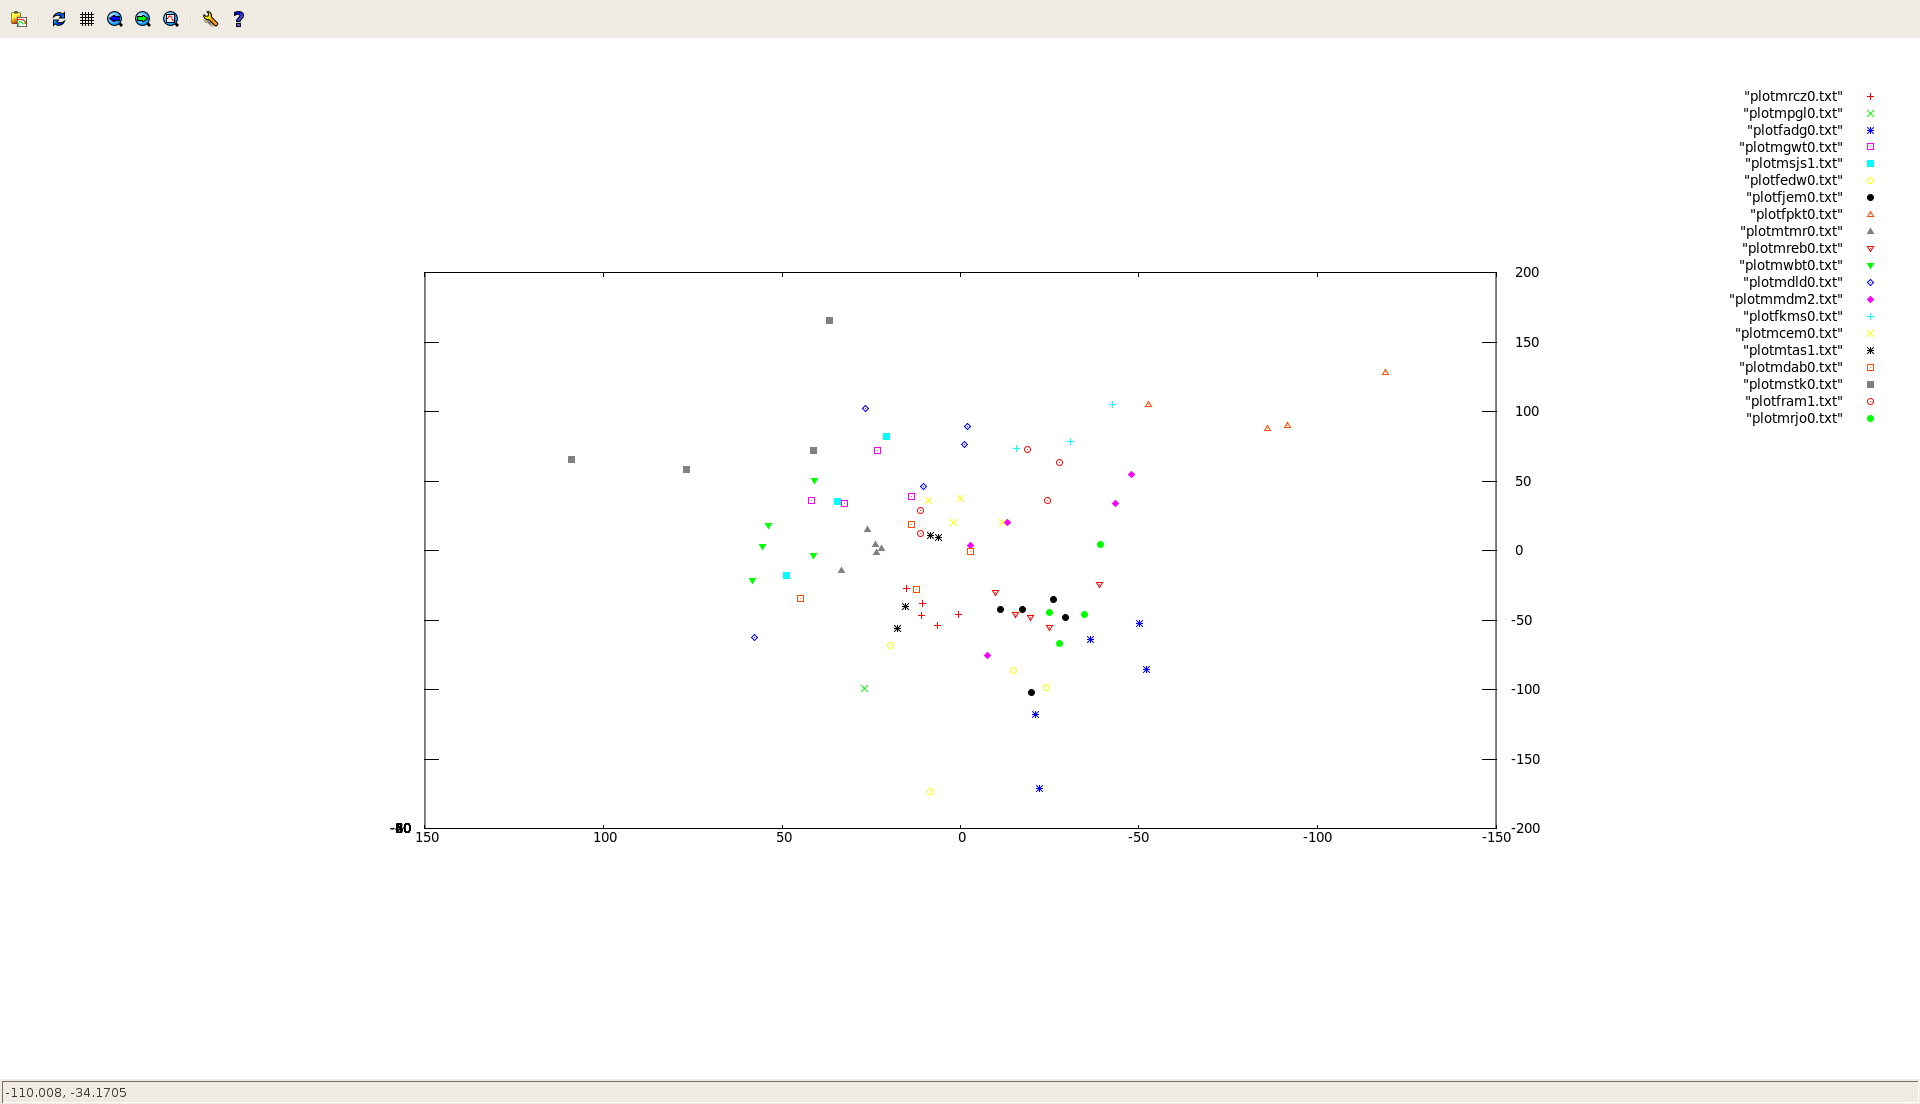
\includegraphics[width=1.00\textwidth]{problem1-fid-pca-1.png}
\caption{Fiduciary Point Offsets In PCA Space}
\label{pca1}
\end{figure}

\begin{figure}
\centering
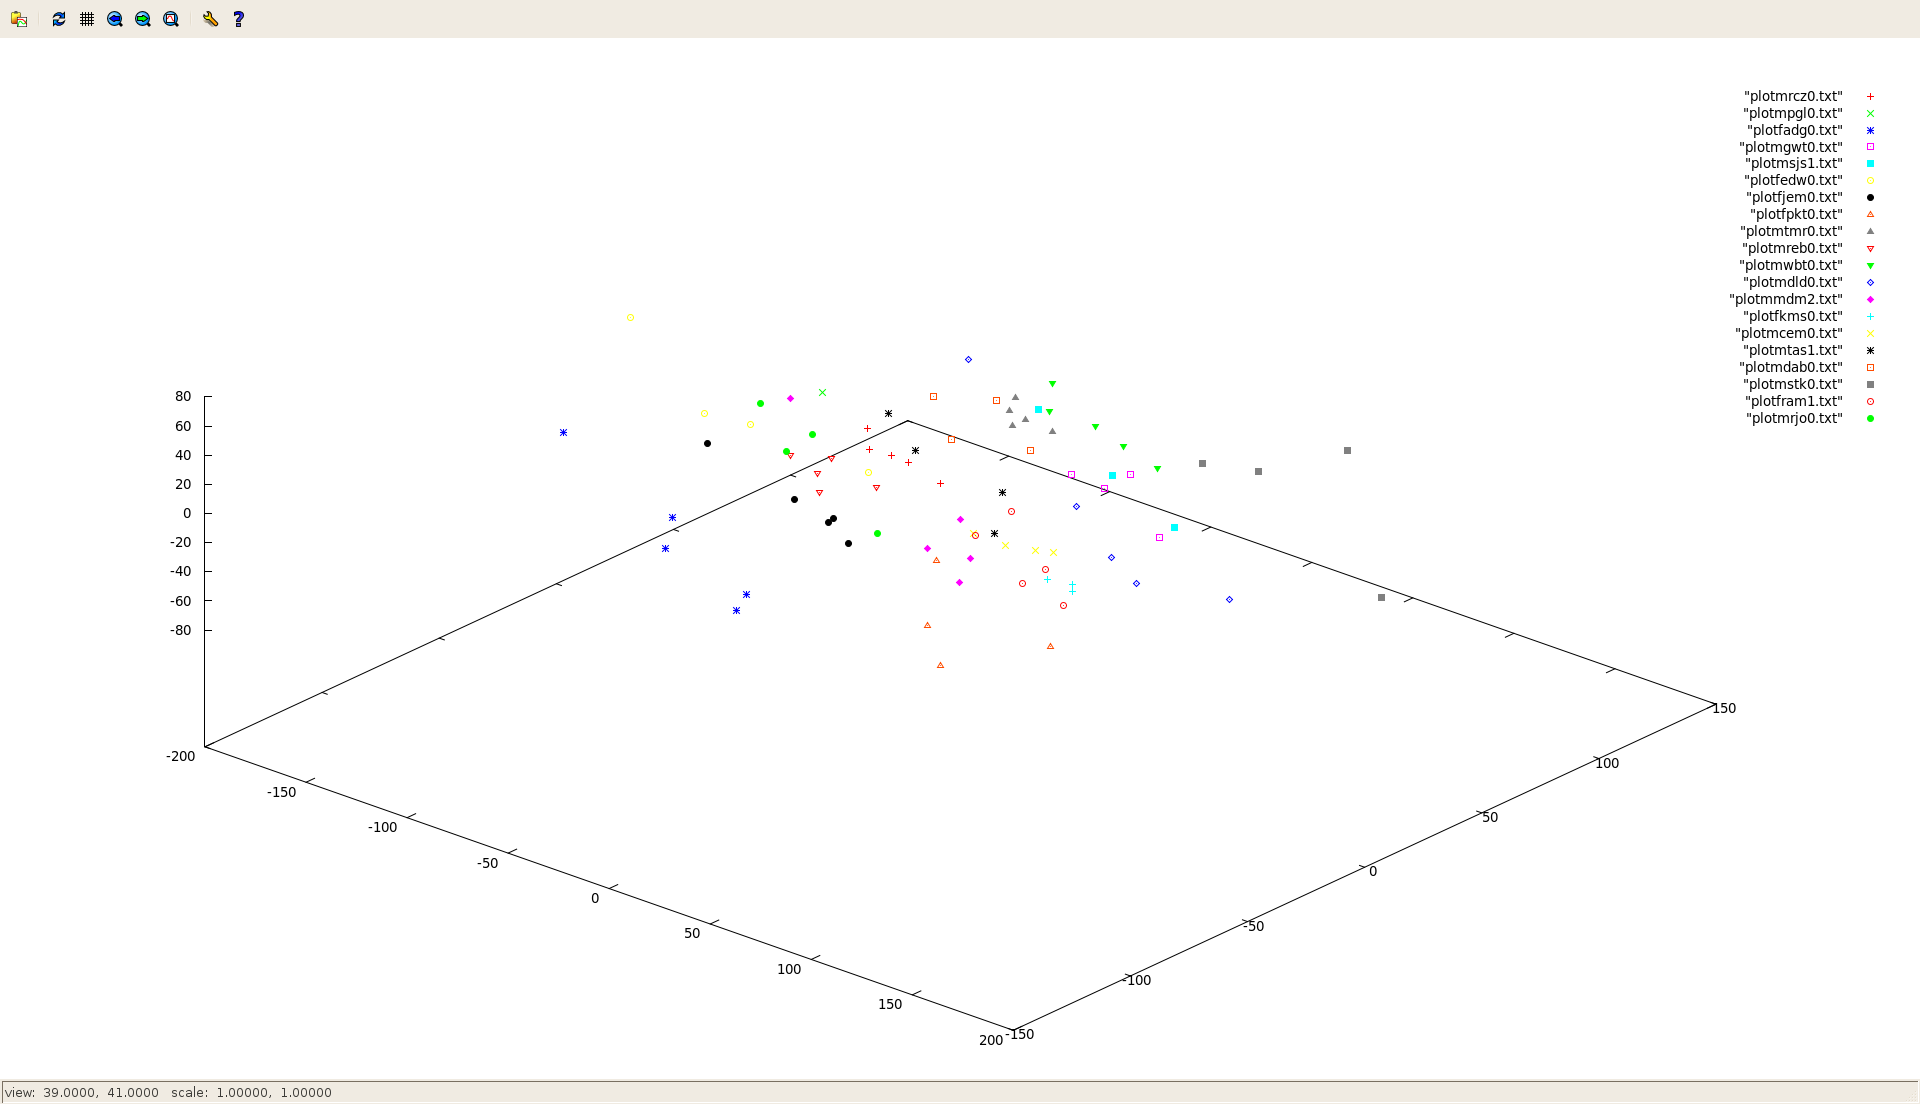
\includegraphics[width=1.00\textwidth]{problem1-fid-pca-2.png}
\caption{Fiduciary Point Offsets In PCA Space (Rotated View)}
\label{pca2}
\end{figure}

To determine the predictive capacity of this recognition system based on fiducial lattices projected into PCA space, leave-one-out cross validation was used. Eighty four different PCA spaces were constructed, each with one data point removed. That data point was then projected into the PCA space and classified using a simple 1-Nearest Neighbor classification. This approach achieved only a 0.36 classification success rate. However, because there are 20 possible people, we would only expect a 0.05 success rate from random guessing.

\end{document}
